\documentclass[12pt, a4paper]{article}
\usepackage{CJKutf8}
\usepackage[left=2cm, right=2cm, top=3cm, bottom=2.5cm]{geometry}
\usepackage[nodayofweek,level]{datetime}
\usepackage{comment}

%..This section controls the header-footer layout of the document
\usepackage{fancyhdr}
\pagestyle{fancy}
\lhead{Machine Learning (NTU CSIE, Fall 2017)}
\chead{}
\rhead{Homework \#2}
\renewcommand{\headrulewidth}{0.4pt}

%..This section controls the title layout
\title{\vspace{-4ex}\bf{\LARGE{Homework \#2}}} 
\author{資工三\space\space\space B04902009\space\space\space 蕭千惠} % \footnote{blablabla} 
\date{\vspace{-2ex}\today\vspace{-4ex}}
%{\formatdate{21}{2}{2017}}

%.. Customize section numbering
%% \setcounter{secnumdepth}{1} % No numbering
%% \setcounter{secnumdepth}{2} % Start numbering
% \renewcommand\thesubsection{(\arabic{subsection})}

\newcommand\BL[2][$\bullet$]{#1\,\parbox[t]{\levelwidth}{\raggedright#2}}
\def\level#1{\unskip $\left\{\vcenter{\hbox{\shortstack{#1}}}\right.$\ignorespaces}
%.. math
\usepackage{mathtools}
\usepackage{amssymb}
\usepackage{amsmath}
\usepackage{upgreek}
\usepackage{bm}

%.. hyperlink / url
\usepackage[hyphens]{url}
\usepackage{hyperref}
\hypersetup{
    colorlinks=true,
    linkcolor=blue,
    filecolor=magenta,      
    urlcolor=blue,
}
\urlstyle{same}
%%\url{url}
%%\herf{url}{words to show}

% .. Include graph
\usepackage{graphicx}
% \includegraphics[width=16.5cm, keepaspectratio=true]{wireless_CSIE_server.png} \par

%.. change font size
\usepackage{type1cm}

%.. change enumerate label
\usepackage{enumitem}
%%\begin{enumerate}[label=(\alph*)]  //(a) (b) (c)
%%\begin{enumerate}[label=(\Alph*)]  //(A) (B) (C)
%%\begin{enumerate}[label=(\roman*)] //(i) (ii) (iii`')
\usepackage{amsfonts}
\usepackage{stmaryrd}

%.. define tab
\newcommand\tab[1][1cm]{\hspace*{#1}}

%.. Content
\begin{document}
	\begin{CJK}{UTF8}{bkai} %use BIG5 enc and bsmi font
	\maketitle\thispagestyle{fancy}
	\linespread{1.5}
	\fontsize{12pt}{18pt} \selectfont

	\section*{Problem 1}
		Score: 200 / 200 \par
		
\includegraphics[width=16.5cm, keepaspectratio=true]{1.png}
	
	\section*{Problem 2}
		The growth function $m_\mathcal{H}(N)$ of positive or negative intervals on $\mathbb{R} = \binom{N+1}{2}+1 = \dfrac{1}{2}N^2+\dfrac{1}{2}N+1$ \\
		We can devide positive-and-negative intervals into two categories:
		\begin{enumerate}
			\item
				The intervals with a leftmost \lq x\rq \space and a positive interval
				$\Rightarrow m_\mathcal{H}(N)= \binom{N}{2}+1$. \\
				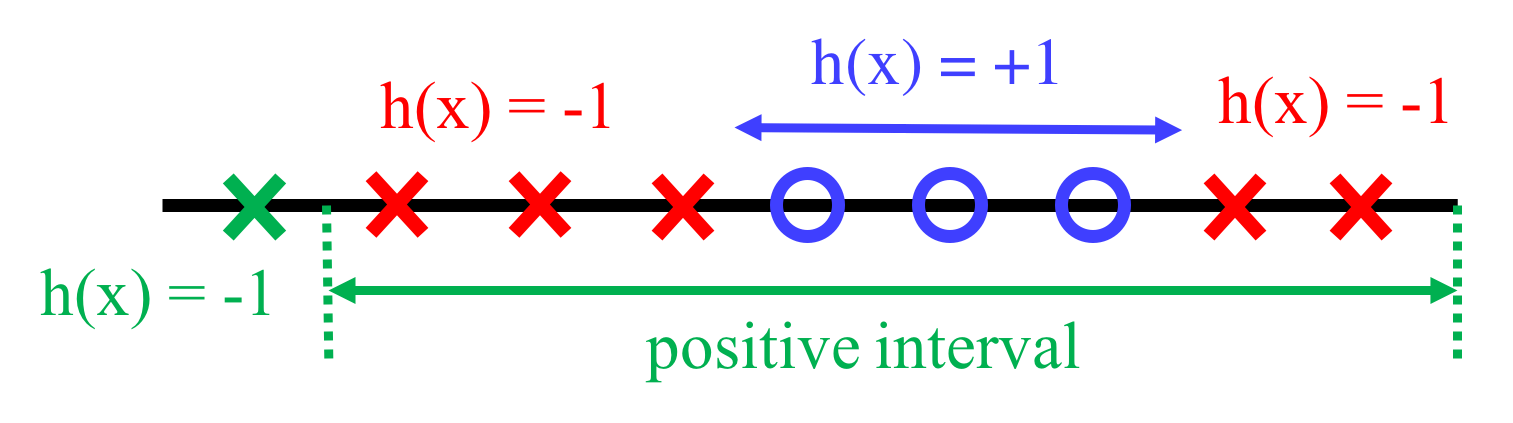
\includegraphics[width=10cm, keepaspectratio=true]{positive.png}
			\item
				The intervals with a leftmost \lq o\rq \space and a negative interval
				$\Rightarrow m_\mathcal{H}(N)= \binom{N}{2}+1$.\\
				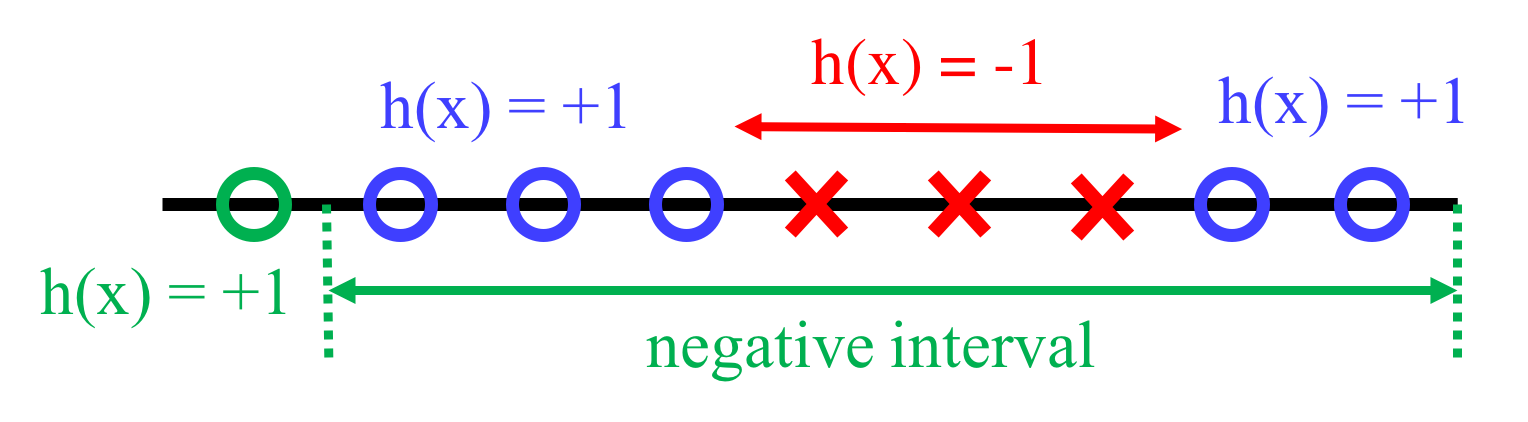
\includegraphics[width=10cm, keepaspectratio=true]{negative.png}
		\end{enumerate}
		The growth function $m_\mathcal{H}(N)$ of positive-and-negative intervals on $\mathbb{R} = 2*(\binom{N}{2}+1) = N^2-N+2$.

	\section*{Problem 3}
		$\mathcal{H} = \Big\{h_c \Big\vert h_c(x) = sign\Big(\sum\limits_{i=0}^{\mathcal{D}}c_ix^i\Big)\Big\}$ \\
		Let $g(x) = \sum\limits_{i=0}^{\mathcal{D}}c_ix^i$ and $a_1, a_2, ..., a_{\mathcal D-1}, a_{\mathcal D}$ be the root of $g(x) \Rightarrow g(x) = \prod\limits_{i=1}^{D}(x-a_i)$\\
		$g$ has $\mathcal{D}+1$ intervals: $(-\infty, a_1], (a_1, a_2],...,(a_{\mathcal{D}-1}, a_{\mathcal{D}}), (a_{\mathcal{D}}, \infty)$ and $g$ alternates sign in the successive intervals. \\
		If $\mathcal{D} = 1$, $\mathcal{H}$ is positive-and-negative rays $\Rightarrow d_{vc}(\mathcal{H}) = 2$\\
		If $\mathcal{D} = 2$, $\mathcal{H}$ is positive-and-negative intervals $\Rightarrow d_{vc}(\mathcal{H}) = 3$ \\
		Let $\mathcal{H}_i$ be the $\mathcal{H}$ with $\mathcal{D} = i$\\
		From the same way described in Problem 2, we conclude that $m_{\mathcal{H}_i}(N)= 2m_{\mathcal{H}_{i-1}}(N)$ \\
		$\Rightarrow d_{vc}(\mathcal{H}_i) = d_{vc}(\mathcal{H}_{i-1})+1$ \\
		$\Rightarrow d_{vc}(\mathcal{H}_\mathcal{D}) = d_{vc}(\mathcal{H}_1)+(\mathcal{D}-1) = 2+(\mathcal{D}-1) = \mathcal{D}+1$ \\
		% $\Rightarrow \mathcal{H}$ is  hypothesis.\\
		$\Rightarrow$ The VC-demension of $\mathcal{H}$ is $\mathcal{D}+1$.

	\section*{Problem 4}
		$\mathcal{H}=\{h_\alpha|h_\alpha(x)=sign(|(\alpha x)\mod4-2|-1),\alpha \in \mathbb{R}\}$\\
		% $\forall t\in \mathbb{R}, \alpha\in\mathbb{R}$
		% $\begin{cases}
		% 	h_\alpha(x)=1$ when $4t-1<\alpha x \leq 4t+1 \\
		% 	h_\alpha(x)=-1$ when $4t+1\leq\alpha x<4t+3 \\
		% \end{cases}$\\
		% 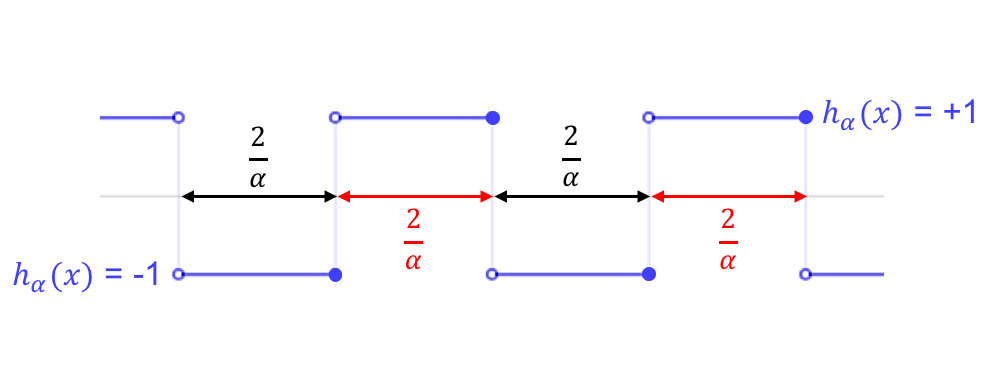
\includegraphics[width=12cm, keepaspectratio=true]{4.png} \\
		Consider N point on $\mathbb{R}$, from 1st point to Nth point, $i^{th}$ point on $4^{i}$ \\
		$\Rightarrow \mathcal{X} = \{4^1, 4^2, ..., 4^{N-1}, 4^N\}$ \\
		Let $\mathcal{Y}$ be a set family containing all $\{+1,-1\}^N$ combinations.\\
		When given an $\alpha$, let's denote the set$\{h_\alpha(x_1), h_\alpha(x_2), ..., h_\alpha(N)\}$ by $y = \{y_1, y_2, ..., y_N\}$\\
		$\forall y \in \mathcal{Y}$, we can find an $\alpha$ to construct it by the pseudocode below.\\
		find\_alpha()\{\\
		\tab $\alpha = 1$ \\
		\tab for($i = 1$; $i \leq N$; $i++$)\\
		\tab \tab if($y_i == -1$)\\
		\tab \tab \tab $\alpha = \alpha + 2 /$pow(4, i)\\
		\tab return $\alpha$\\
		\}\\
		When $\alpha = 1$, $\forall x \in \mathcal{X}, h_\alpha(x) = +1$\\
		When flipping $x_i$ from +1 to -1, we add $\dfrac{2}{4^i}$ to $\alpha$.\\
		To proof that adding $\dfrac{2}{4^i}$ to $\alpha$ will only affect the point $x_i$, we divided all $x\in\mathcal{X}$ into three cases:
		\begin{enumerate}
		\item {\bf $\bm{x_j}$ with $\bm{1\leq j < i}$}\\
			We have to proof that flipping all points larger than $x_j$ won't affect the value of $y_j$. \\
			To flip all points larger than $x_j$, $\alpha = 1 + \sum\limits_{k = j+1}^{n} \dfrac{2}{4^k} = 1 + \dfrac{2}{3*4^j}[1-(\dfrac{1}{4})^{n-j+1}]$\\
			$\alpha x_j = \{1+\dfrac{2}{3*4^j}[1-(\dfrac{1}{4})^{n-j+1}]\} * 4^j = 4^j+\dfrac{2}{3}[1-(\dfrac{1}{4})^{n-j+1}] < 4^j+\dfrac{2}{3}$\\
			$\Rightarrow  sign(|(\alpha x_j)\mod 4-2|-1) = +1$\\
			$\Rightarrow y_j$ remains the same.
		\item {$\bm{x_i}$}\\
			$\dfrac{2}{4^i} x_i = \dfrac{2}{4^i}*4^i = 2$\\
			$\Rightarrow y_i = sign(|(\dfrac{2}{4^i} x_i)\mod 4-2|-1) = sign(|2\mod4-2|-1) = -1$
		\item {\bf $\bm{x_j}$ with $\bm{i < j \leq N}$}\\
			$x_j = x_i * 4^{j-i}$\\
			$(\dfrac{2}{4^i}*x_j)\mod 4 = (\dfrac{2}{4^i}*x_i*4^{j-i})\mod 4 = 0$ \\
			$\Rightarrow y_j$ remains the same.
		\end{enumerate}
		Since all $\{+1,-1\}^N$ combinations can be constructed, $\mathcal{H}$ can shatter any N.\\
		$\Rightarrow$ The VC-demension of $\mathcal{H}$ is $\infty$.

	\section*{Problem 5}
		\begin{enumerate}
		\item
			$\forall N < d_{vc}(\mathcal{H}_1),$ any N inputs can be shattered by $\mathcal{H}_1$. \\
			Since $\mathcal{H}_1 \subseteq \mathcal{H}_2$, any N inputs can be shattered by $\mathcal{H}_2$ 
			$\Rightarrow d_{vc}(\mathcal{H}_1) \ngtr d_{vc}(\mathcal{H}_2)$
		\item
			When $\mathcal{H}_1 = \mathcal{H}_2, d_{vc}(\mathcal{H}_1) = d_{vc}(\mathcal{H}_2)$
		\item
			Let $\mathcal{H}_1$ be positive interval hypothesis $\Rightarrow d_{vc}(\mathcal{H}_1) = 2$  (Known from the course slide.)\\
			Let $\mathcal{H}_2$ be positive-and-negative intervals hypothesis. \\
			$\Rightarrow m_{\mathcal{H}_2}(N)= N^2-N+2$ (Known from Problem 2) $\Rightarrow d_{vc}(\mathcal{H}_2) = 3$\\
			$\mathcal{H}_1 \subseteq \mathcal{H}_2$ and $d_{vc}(\mathcal{H}_1) < d_{vc}(\mathcal{H}_2)$
		\end{enumerate}
		From 1 \& 2 \& 3 $\Rightarrow$ $d_{vc}(\mathcal{H}_1) \leq d_{vc}(\mathcal{H}_2)$

	\section*{Problem 6}
		$\mathcal{H}1 \cup \mathcal{H}2 =$ the positive-and-negative ray set. \\
		The growth function $m_{\mathcal{H}1 \cup \mathcal{H}2}(N)$ of positive-and-negative ray on $\mathbb{R} = 2(N+1)-2 = 2N$. \\
		$m_{\mathcal{H}1 \cup \mathcal{H}2}(N) = 2N \neq 2^N$ when $N > 3$ \\
		$\Rightarrow$ The VC-demension of $\mathcal{H}1 \cup \mathcal{H}2$ is 2.
	
	\fontsize{12pt}{20pt} \selectfont
	\section*{Problem 7}
		% $err(h_{s,\theta}({\bf x}), f({\bf x})) = \llbracket \tilde{y} \neq y \rrbracket$\\
		$P(y|{\bf x}) = 
		\begin{cases}
			0.8, y = f({\bf x}) \\
			0.2, y \neq f({\bf x}) \\
		\end{cases}$\\
		Let $h_{s,\theta}$ makes an error with probability $\mu$. ($P(h_{s,\theta}({\bf x}) \neq f({\bf x}))=\mu$)  \\
		\begin{tabular}[t]{|c|c|c|}
			\hline
			$\mu$ 	& $\theta > 0$ 			& $\theta < 0$ \\
			\hline
			s = 1   	& $\dfrac{\theta}{2}$   & $\dfrac{|\theta|}{2}$ \\
			\hline
			s = -1   	& $1-\dfrac{\theta}{2}$	& $1-\dfrac{\theta}{2}$ \\
			\hline
		\end{tabular}\par
		\vspace{0.5em}\noindent
		$\Rightarrow$ When s = 1, $\mu = \dfrac{|\theta|}{2}$. When s = -1, $\mu = 1-\dfrac{|\theta|}{2}$ \\
		$\mu = \dfrac{s+1}{2} \dfrac{|\theta|}{2} + \dfrac{1-s}{2}(1-\dfrac{|\theta|}{2})
			 = \dfrac{1-s+s|\theta|}{2}$\\
		$E_{out}(h_{s,\theta}) = 0.8\mu+0.2(1-\mu)= 0.5+0.3s(|\theta|-1)$

	\fontsize{12pt}{10pt} \selectfont
	\section*{Problem 8}
		Findings: 
		\begin{enumerate}
		\item 
			The smaller the $E_{in}$ is, the smaller the maximum $E_{out}$ is.
		\item 
			$P(E_{in}=0.2) = 0.41$\\
			$\Rightarrow E_{in} = 0.2$ most frequently occured since $P(y|{\bf x}) = 0.2$ when $y \neq f({\bf x})$.
		\end{enumerate}
		Averaged $E_{in} = 0.150450$, Averaged $E_{out} = 0.243626$\\
		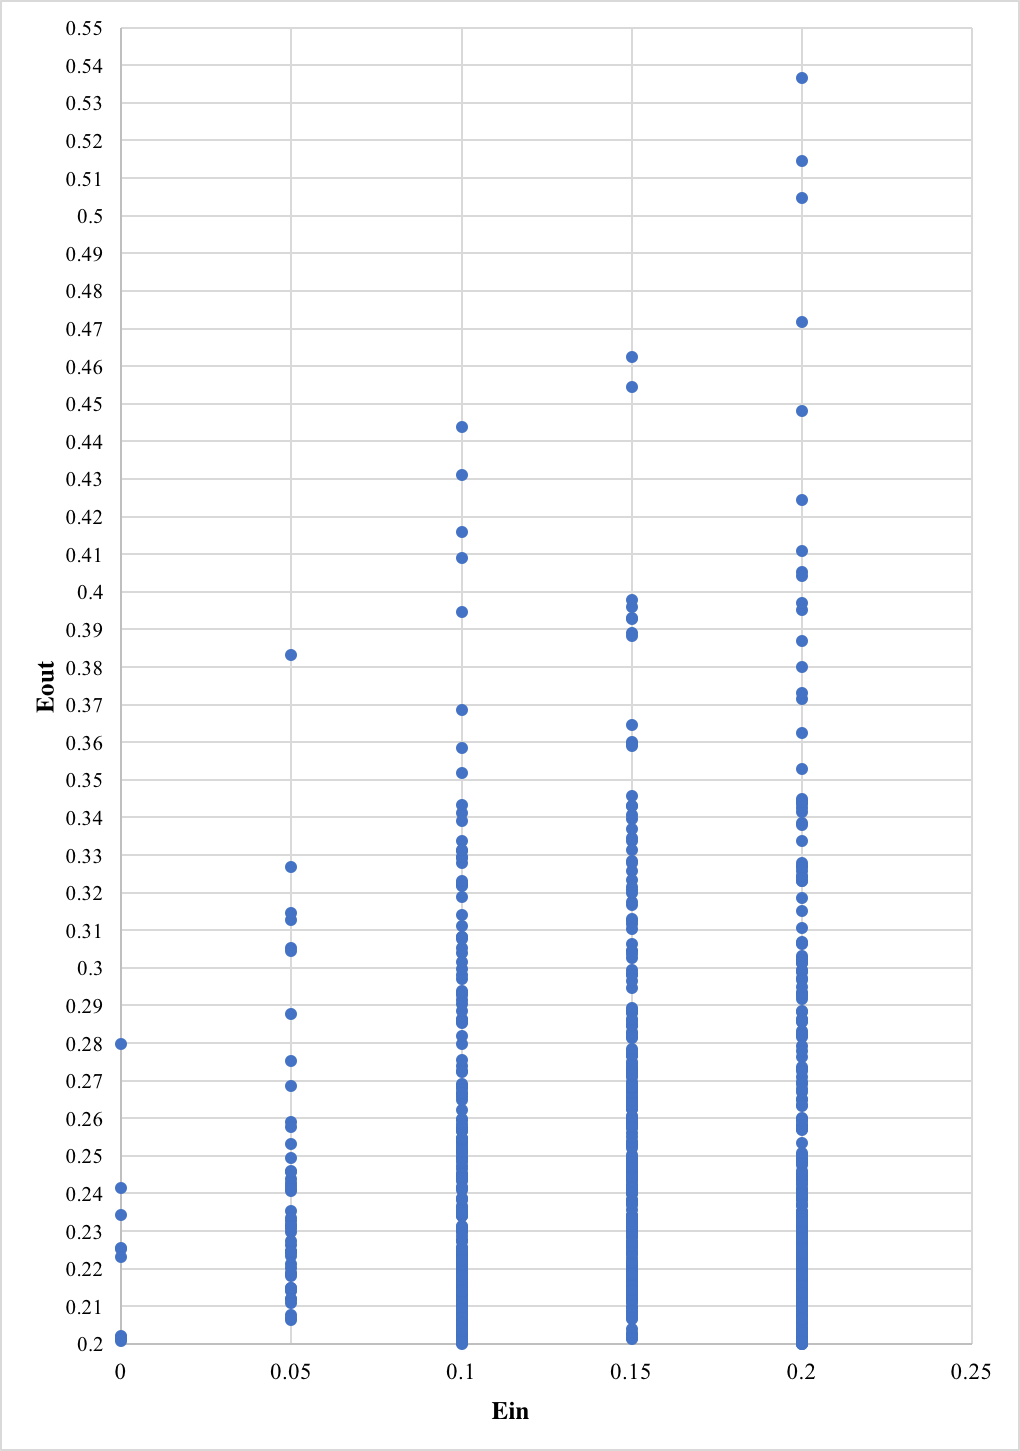
\includegraphics[width=17cm, keepaspectratio=true]{8.png} \par
	
	\fontsize{12pt}{15pt} \selectfont
	\section*{Problem 9(Bonus)}
		% The VC-dimension of perceptron learning model in d dimensions is d+1. \\
		% $\Rightarrow$ The break point of perceptron learning model in d dimensions is d+2.\\
		% $\Rightarrow \begin{cases}
		% 	m_\mathcal{H}(N) = O(N^{d+1}) \\
		% 	\forall n\in\mathbb{Z} \land 0 \leq n\leq d+1 , m_\mathcal{H}(n) = 2^n \\
		% \end{cases}$\\
		% Let $m_\mathcal{H}(N) = \sum\limits_{i=0}^{d+1} a_i N^i$.\\
		% With d+1 pairs of $(n, m_\mathcal{H}(n))$ be given, we can find out all $a_i$ $(0 \leq i \leq d+1)$ and solve $m_\mathcal{H}(N)$.\\
		% $\forall n\in\mathbb{Z} \land 0 \leq n\leq d+1 , m_\mathcal{H}(n) = 2^n  = 2*2^{n-1}= 2(1+1)^{n-1} = 2\sum\limits_{i=0}^{n-1} \binom{n-1}{i}$
		% When 
		% $\begin{cases}
		% 	n = d+1, m_\mathcal{H}(n) = 2\sum\limits_{i=0}^{d}\binom{n-1}{i} \\
		% 	0 \leq n \leq d, \sum\limits_{i=0}^{n-1} \binom{n-1}{i} = \sum\limits_{i=0}^{n-1} \binom{n-1}{i} + \sum\limits_{i=n}^{d} \binom{n-1}{i} {\color{blue} \pmb=} \sum\limits_{i=0}^{d} \binom{n-1}{i}
		% 	\Rightarrow m_\mathcal{H}(n) = 2\sum\limits_{i=0}^{n-1} \binom{n-1}{i} = 2\sum\limits_{i=0}^{d} \binom{n-1}{i}
		% \end{cases}$ \par
		% \hspace{10em}{\color{blue} \bf(Since ${\bf \binom{a}{b} = 0}$ when ${\bf a < b \Rightarrow \sum\limits_{i=n}^{d} \binom{n-1}{i} = \sum\limits_{i=n}^{d} 0 = 0}$)}\\
		% $\Rightarrow m_\mathcal{H}(N) = 2\sum\limits_{i=0}^d \binom{N-1}{i}$		
		Let's denote the growth function for perceptron learning model in $d$ dimensions with $N$ points by $m_{\mathcal{H}, d}(N)$. \\
		We will find an expression for $m_{\mathcal{H}, d}(N)$ through induction. \\
		First imaging having N-1 points and then we add one more point. \\
		The linearly separable partitions of the previous $N-1$ points can be separated into two cases:
		\begin{enumerate}
		\item
			{\bf There is a separating hyperplane for the previous $N-1$ points passing through the new point:} each such linearly separable partition of the previous $N-1$ points gives rise to two distinct linearly separable partitions when the new point is added as the hyperplane can be shifted infinitesimally to place the new point in either class.
			(Let's denotes the number of linearly separable partitions of the previous $N-1$ points in this case by $P_1$.)
		\item
			{\bf There is no separating hyperplane passing through the new point:} each such linearly separable partition gives rise to only one linearly separable partition when the new point is added.
			(Let's denotes the number of linearly separable partitions of the previous $N-1$ points in this case by $P_2$.)
		\end{enumerate}
		$m_{\mathcal{H}, d}(N) = 2P_1+P_2 = (P_1+P_2)+P_1 = m_{\mathcal{H}, d}(N-1)+P_1$\\
		Restricting the separating hyperplane to go through a particular point is the same as eliminating one degree of freedom and thus projecting the previous $N-1$ points to a $(d-1)$-dimensional space. Therefore, we can know that $P_1 = m_{\mathcal{H}, d-1}(N-1)$\\
		$\Rightarrow m_{\mathcal{H}, d}(N)$ = $m_{\mathcal{H}, d}(N-1)+m_{\mathcal{H}, d-1}(N-1)$ \\
		By recursive: $m_{\mathcal{H}, d}(N) = \binom{N-1}{0}m_{\mathcal{H}, d}(1)+\binom{N-1}{1}m_{\mathcal{H}, d-1}(1)+...+\binom{N-1}{N-1}m_{\mathcal{H}, d-N+1}(1)$\\
		$m_{\mathcal{H}, d}(1) = 0$ when $d < 0$, otherwise $m_{\mathcal{H}, d}(1) = 1$\\
		$\begin{cases}
			\forall d < N-1,  m_{\mathcal{H}, d}(N) = \binom{N-1}{0}m_{\mathcal{H}, d}(1)+\binom{N-1}{1}m_{\mathcal{H}, d-1}(1)+...+\binom{N-1}{d}m_{\mathcal{H}, 0}(1) = 2\sum\limits_{i=0}^d \binom{N-1}{i}\\
			\forall d \geq N-1, m_{\mathcal{H}, d}(N) = 2\sum\limits_{i=0}^{N-1} \binom{N-1}{i} {\color{blue} \pmb=} 2\sum\limits_{i=0}^d \binom{N-1}{i} \\
		\end{cases}$\par
		\hspace{12em}{\color{blue} \bf(Since ${\bf \binom{a}{b} = 0}$ when ${\bf a < b \Rightarrow \binom{N-1}{i} = 0}$ when $N \leq i \leq d$)}\\
		$\Rightarrow m_{\mathcal{H}, d}(N) = 2\sum\limits_{i=0}^d \binom{N-1}{i}$ \\
		

	\clearpage
	\end{CJK}
\end{document}